% Created 2021-02-03 三 00:24
% Intended LaTeX compiler: pdflatex
\documentclass[11pt]{article}
\usepackage[utf8]{inputenc}
\usepackage[T1]{fontenc}
\usepackage{graphicx}
\usepackage{grffile}
\usepackage{longtable}
\usepackage{wrapfig}
\usepackage{rotating}
\usepackage[normalem]{ulem}
\usepackage{amsmath}
\usepackage{textcomp}
\usepackage{amssymb}
\usepackage{capt-of}
\usepackage{hyperref}
\setcounter{secnumdepth}{3}
\author{Steiner}
\date{\today}
\title{套接字错误处理}
\hypersetup{
 pdfauthor={Steiner},
 pdftitle={套接字错误处理},
 pdfkeywords={},
 pdfsubject={},
 pdfcreator={Emacs 26.3 (Org mode 9.1.9)}, 
 pdflang={English}}
\begin{document}

\maketitle
\tableofcontents


\section{套接字程序中遇到的错误}
\label{sec:org80e9d22}
\begin{center}
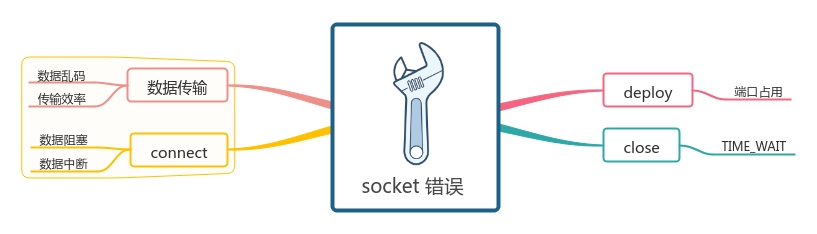
\includegraphics[width=.9\linewidth]{./images/socket-debug.jpg}
\end{center}

套接字编程中遇到的错误,可以通过发生的场景分为4部分,与前文的四步骤一一对应\\
\subsection{部署时遇到的错误}
\label{sec:org054ed6a}
\subsubsection{地址已占用}
\label{sec:orgd43f1cc}
关闭服务端套接字时,服务端所使用的端口状态还是 \textbf{TIME\_WAIT} ,端口还在被占用\\
再次启动服务端程序时,会发现 \emph{address already in use}\\

要解决这个问题,只需在服务端套接字 \emph{bind} 前,\\
设置 \emph{SO\_REUSEADDR} 属性\\
\begin{verbatim}
int on = 1;
setsockopt(sockfd, SOL_SOCKET, SO_REUSEADDR, &on, sizeof(on));
\end{verbatim}
\subsection{连接时遇到的错误}
\label{sec:orgfc67767}
\begin{center}
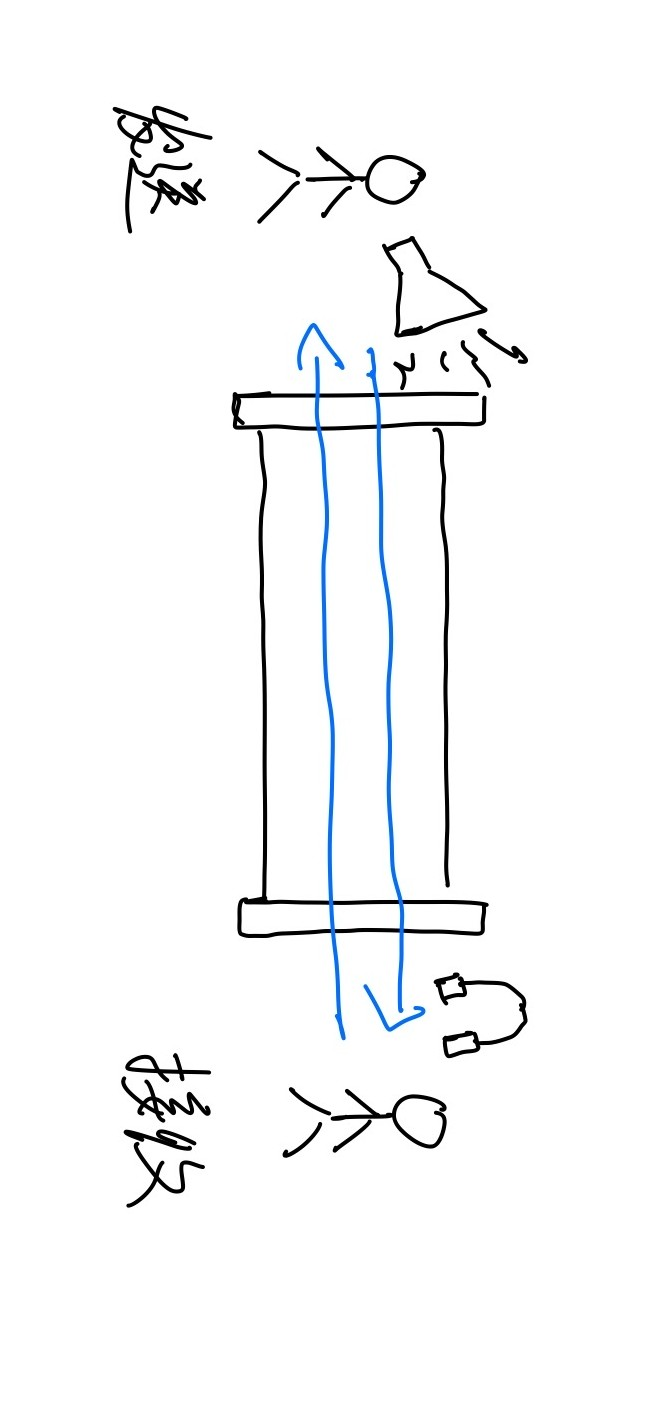
\includegraphics[width=.9\linewidth]{./images/socket.jpg}
\end{center}
\emph{connect} 与 \emph{accept} 连接了两个套接字,这里看作两个套接字之间有一个管道将他们相连\\

那么遇到的问题可以分为\\
\subsubsection{数据阻塞}
\label{sec:org9c37d77}
数据传输的阻塞有可能是网络的问题,也有可能是电脑死机无法响应数据,\\

这个时候我们可以在对端为 \emph{read} 设置超时时间\\
\begin{verbatim}
struct timeval tv;
tv.tv_sec = 5;
tv.tv_usec = 0;
setsockopt(connfd, SOL_SOCKET, SO_RCVTIMEO, (const char *) &tv, sizeof tv);
\end{verbatim}

也可以在轮询的时候设置超时,这里先不做探讨\\

然后我该怎么知道是发生了超时事件 ??\\
此时/read/ 返回 -1, 并且 \emph{errno} 为 \emph{EAGAIN} 或 \emph{EWOULDBLOCK}\\
\textbf{\textbf{tips}}\\
鬼知道这两个错误码什么意思,先用着好了\\

\subsubsection{数据中断}
\label{sec:orge9eb92b}
此时维持双方数据传输的通道断裂,可能是由于程序崩溃引起的\\
此时在崩溃的一方,操作系统回收资源,自动调用 \emph{shutdown}  \\

若 \textbf{数据发送端} 没有崩溃,调用 \emph{write} 时触发 \emph{SIGPIPE} 信号,\\
此时返回值为 \textbf{-1},并且 \emph{errno = EPIPE}\\

若 \textbf{数据接收端} 没有崩溃, 调用 \emph{read} 时会接收到 \emph{EOF} 信号,返回值为 \textbf{0}\\

遇到这种情况只能先手动关闭连接了\\
\textbf{\textbf{tips}}\\
遇到 \emph{SIGPIPE} 时,程序一般会退出,如果不想退出可以调用\\
\begin{verbatim}
signal(SIGPIPE, SIG_IGN); // SIG_IGN: signal ignore
\end{verbatim}
\subsection{传输数据时遇到的错误}
\label{sec:orgb44ba17}
\subsubsection{数据乱码}
\label{sec:org7b1c549}
\begin{quote}
不同的CPU有不同的字节序类型 这些字节序是指整数在内存中保存的顺序 这个叫做主机序\\
\end{quote}

怕什么,整数的问题关我字节流什么事,直接把数据指针强制转化为 \emph{const char *} 发送即可\\
\begin{verbatim}
send(connfd, (const char *)&data, sizeof(data), 0);
\end{verbatim}
\subsubsection{{\bfseries\sffamily TODO} 传输效率过低}
\label{sec:org3d4d8e6}
要传输的数据量太小,就像澡堂里就一个人洗澡,老板得陪死\\
为了解决这个问题,我们可以用 \emph{writev} 与 \emph{readv} 函数来处理数据读写\\
这两个函数可以 \textbf{聚集写} , \textbf{散布读}\\
\begin{verbatim}
#include <sys/uio.h>
ssize_t readv(int fd, const struct iovec *iov, int iovcnt);
ssize_t writev(int fd, const struct iovec *iov, int iovcnt);
\end{verbatim}
但我好像不会用啊\\
\subsection{关闭}
\label{sec:org5d4cf12}
好像没有诶\\
\end{document}